\documentclass[12pt,x11names,a4paper]{article}
\input{preamble}


\newgeometry{margin=2cm}

\pagestyle{fancy}
\fancyhf{}

\rhead{Nørre Gymnasium\\2.z
}
\cfoot{Side \thepage \hspace{1pt} af \pageref{LastPage}}

%Husk at rette modul og dato!
\lhead{Aflevering 4\\ Matematik B
}
\chead{13. december
}

\begin{document}

%
\includepdf[pages=-]{Forsider/aarsprove_1v.pdf}
\savegeometry{art}

\begin{titlepage}
\newgeometry{margin=0pt}

\begin{minipage}{0.27\textwidth}

\begin{tikzpicture}[overlay]
\fill[top color = NorregGroen!40, bottom color = NorregGroen] (6,10) rectangle (-10,-30);
\end{tikzpicture}
\end{minipage}
\begin{minipage}{0.73\textwidth}
\begin{center}
\phantom{h} \vspace{1cm}\\
\hspace{4cm}

\includegraphics[scale = 1]{Billeder/Norreg.png} \\
\phantom{h} \vspace{5cm}\\
\rule{0.7\textwidth}{0.3mm}\\
\phantom{h}\\
{\fontsize{50}{60}\selectfont Aflevering 4}\\
\phantom{h}\\
\rule{0.7\textwidth}{0.3mm}\\
\Large 2024\\
\Large 2.z Ma

\end{center}
\end{minipage}
\end{titlepage}
\loadgeometry{art}

%Udfyld afsnit herunder og lav til egen Latex-fil

%Kopier følgende til overskrift:

%\begin{center}
%\Huge
%Aflevering 1
%\end{center}
%\section*{Opgave 1}
%\stepcounter{section}
\begin{center}
%Opgavesætter er delt i to dele:\\
%Delprøve 1 kun med den centralt udmeldte formelsamling.\\
%Delprøve 2 med alle hjælpemidler.
\end{center}

\section*{Krav til formidling af din besvarelse}

Ved bedømmelse af helhedsindtrykket af besvarelsen af de enkelte opgaver lægges særlig vægt på følgende fire punkter:
\begin{itemize}
\item[$\cdot$] \textbf{Redegørelse og dokumentation for metode} \\
Besvarelsen skal indeholde en redegørelse for den anvendte løsningsstragegi med dokumentation i form af et passende antal mellemregninger \textit{eller} matematiske forklaringer på metoden, når et matematisk værktøjsprogram anvendes.
\item[$\cdot$] \textbf{Figurer, grafer og andre illustrationer} \\
Besvarelsen skal indeholde hensigtsmæssig brug af figurer, grafer og andre illustrationer, og der skal være tydelige henvisninger til brug af disse i den forklarende tekst.
\item[$\cdot$] \textbf{Notation og layout}\\
Besvarelsen skal i overensstemmelse med god matematisk skik opstilles med hensigtsmæssig brug af symbolsprog, og med en redegørelse for den matematiske notation, der indføres og anvendes, og som ikke kan henføres stil standardviden.
\item[$\cdot$] \textbf{Formidling og forklaring}\\
Besvarelsen af rene matematikopgaver skal indeholde en angivelse af givne oplysninger og korte forklaringer knyttet til den anvendte løsningsstrategi beskrevet med brug af almindelig matematisk notation. 

Besvarelsen af opgaver, der omhandler matematiske modeller, skal indeholde en kort præsentation af modellens kontekst, herunder betydning af modellens parametre. De enkelte delspørgsmål skal afsluttes med en præcis konklusion præsenteret i et klart sprog i relation til konteksten.
\end{itemize}

\newpage



\begin{center}
\LARGE
Delprøve uden hjælpemidler 
\end{center}
\stepcounter{section}

%%%%%%%%%%%%%%%%%%%%%%%%%%
%
%
%
%
%%%%%%%%%%%%%%%%%%%%%%%%%%
\begin{opgavetekst}{Opgave 1}
	En funktion $g$ givet ved forskriften
	\begin{align*}
		g(x) = b\cdot a^x
	\end{align*}
	opfylder, at $g(1) = 5$ og $g(4) = 40$.
\end{opgavetekst}
\begin{delopgave}{}{1}
	Bestem en forskrift for $g$. 
\end{delopgave}
\begin{delopgave}{}{2}
	Bestem $g(2)$
\end{delopgave}
%%%%%%%%%%%%%%%%%%%%%%%%%%
%
%
%
%
%%%%%%%%%%%%%%%%%%%%%%%%%%
\begin{opgavetekst}{Opgave 2}
	To funktioner $f$ og $g$ er givet ved
	\begin{align*}
		f(x) = x^2-2x+13
	\end{align*}
	og 
	\begin{align*}
		g(x) = \log_2(x).
	\end{align*}
\end{opgavetekst}
\begin{delopgave}{}{1}
	Opskriv forskriften for den sammensatte funktion $h(x) = g(f(x))$.
\end{delopgave}
\begin{delopgave}{}{2}
	Bestem $h(3)$.
\end{delopgave}
%%%%%%%%%%%%%%%%%%%%%%%%%%
%
%
%
%
%%%%%%%%%%%%%%%%%%%%%%%%%%
\begin{opgavetekst}{Opgave 3}
	På Figur \ref{fig:potens} ses grafen for en potensfunktion $f$ givet ved
	\begin{align*}
		f(x) = b\cdot x^{a}
	\end{align*}
	\begin{figure}[H]
		\centering
		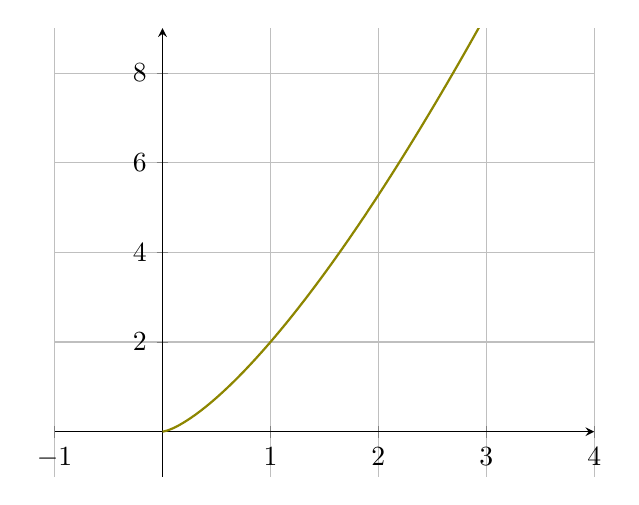
\begin{tikzpicture}
			\begin{axis}
			[ axis lines = center,
			xmin = -1, xmax = 4,
			ymin = -1, ymax = 9,
			grid = major,
			]
				\addplot[color = olive, thick, samples = 100, domain = 0:5] {2*x^(1.4)};
			\end{axis}
		\end{tikzpicture}
		\caption{Graf for funktionen $f$.}
		\label{fig:potens}
	\end{figure}
	\phantom{h}
\end{opgavetekst}
\begin{delopgave}{}{1}
	Bestem tallet $b$.
\end{delopgave}
\begin{meretekst}
	Det oplyses, at $a$ er enten $1.4$, $0.7$ eller $-0.7$. 
\end{meretekst}
\begin{delopgave}{}{2}
	Afgør værdien af $a$. 
\end{delopgave}
\newpage

\begin{opgavetekst}{Opgave 4}
	En funktion $f$ er givet ved
	\begin{align*}
		f(x) = \frac{1}{3}x^3 + \frac{1}{2}x^2 - 6x + 2
	\end{align*}
\end{opgavetekst}

\begin{delopgave}{}{1}
	Løs ligningen $f'(x) = 0$.
\end{delopgave}
\begin{delopgave}{}{2}
	Bestem monotoniforholdene for $f$. 
\end{delopgave}

\begin{opgavetekst}{Opgave 5}
	En funktion $h$ er givet ved
	\begin{align*}
		h(x) = 2\sqrt{x} + x^2
	\end{align*}
\end{opgavetekst}
\begin{delopgave}{}{1}
	Bestem en ligning for tangenten til $h$ i punktet $(4,h(4))$.
\end{delopgave}


\newpage

\begin{center}
\LARGE
Delprøve med hjælpemidler 
\end{center}
\stepcounter{section}

\begin{opgavetekst}{Opgave 6}
	\begin{center}
		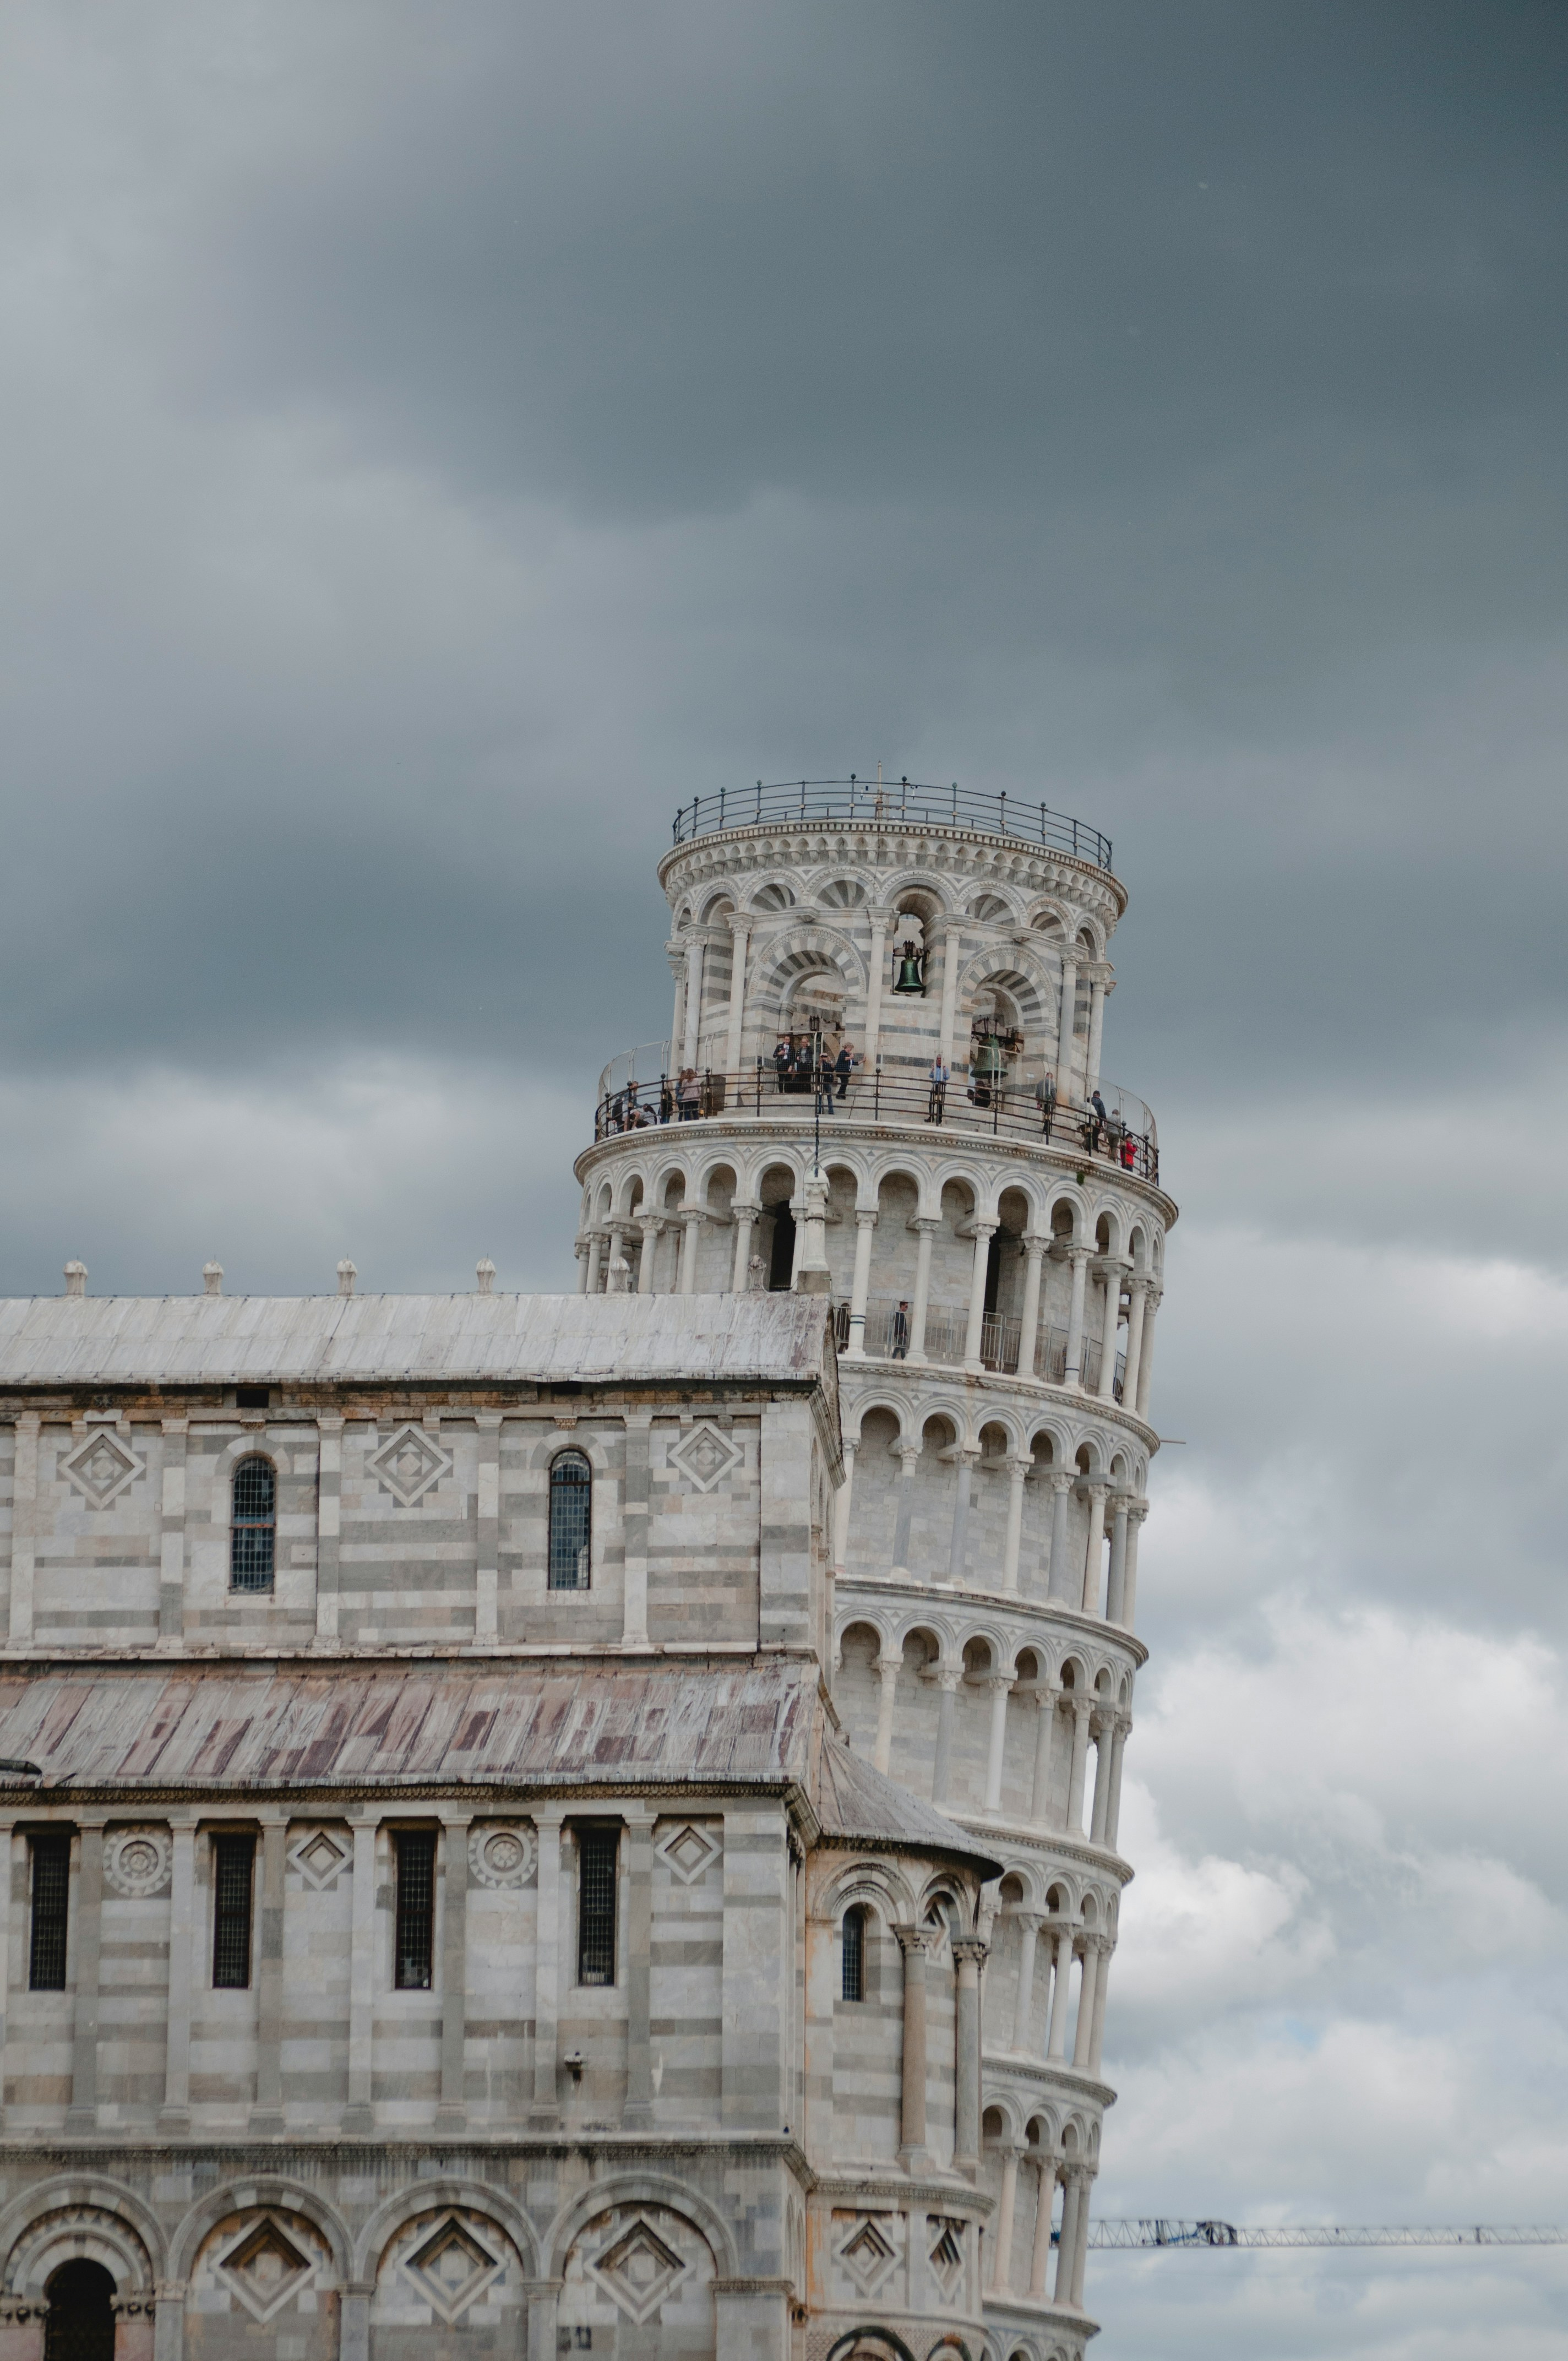
\includegraphics[width=0.6\textwidth]{Billeder/pisa}
	\end{center}
	Tegner vi en vektor $\vv{v}$ fra jordoverfladen langs undersiden af det skæve tårn i Pisa, så vil vektoren 
	have koordinater
	\begin{align*}
		\vv{v} = 
		\begin{pmatrix}
			3.88 \\
			55.86
		\end{pmatrix}.
	\end{align*}	 
\end{opgavetekst}
\begin{delopgave}{}{1}
	Bestem højden af tårnet, hvis det ikke var skævt. 
\end{delopgave}
\begin{meretekst}
	En vektor langs jorden må lyde 
	\begin{align*}
		\vv{u} = 
		\begin{pmatrix}
			1 \\ 0
		\end{pmatrix}.
	\end{align*}
\end{meretekst}
\begin{delopgave}{}{2}
	Bestem koordinatsættet til projektionsvektoren
	\begin{align*}
		\vv{v_{\vv{u}}}.
	\end{align*}
\end{delopgave}
\begin{meretekst}
	Længden af denne vektor må være lig den vandrette afstand, som tårnets top har fra tårnets bund. Det er 
	altså længden af tårnets udhæng.
\end{meretekst}
\begin{delopgave}{}{3}
	Bestem længden af tårnets udhæng. Kender vi allerede dette tal?
\end{delopgave}


\begin{opgavetekst}{Opgave 7}
	\begin{center}
		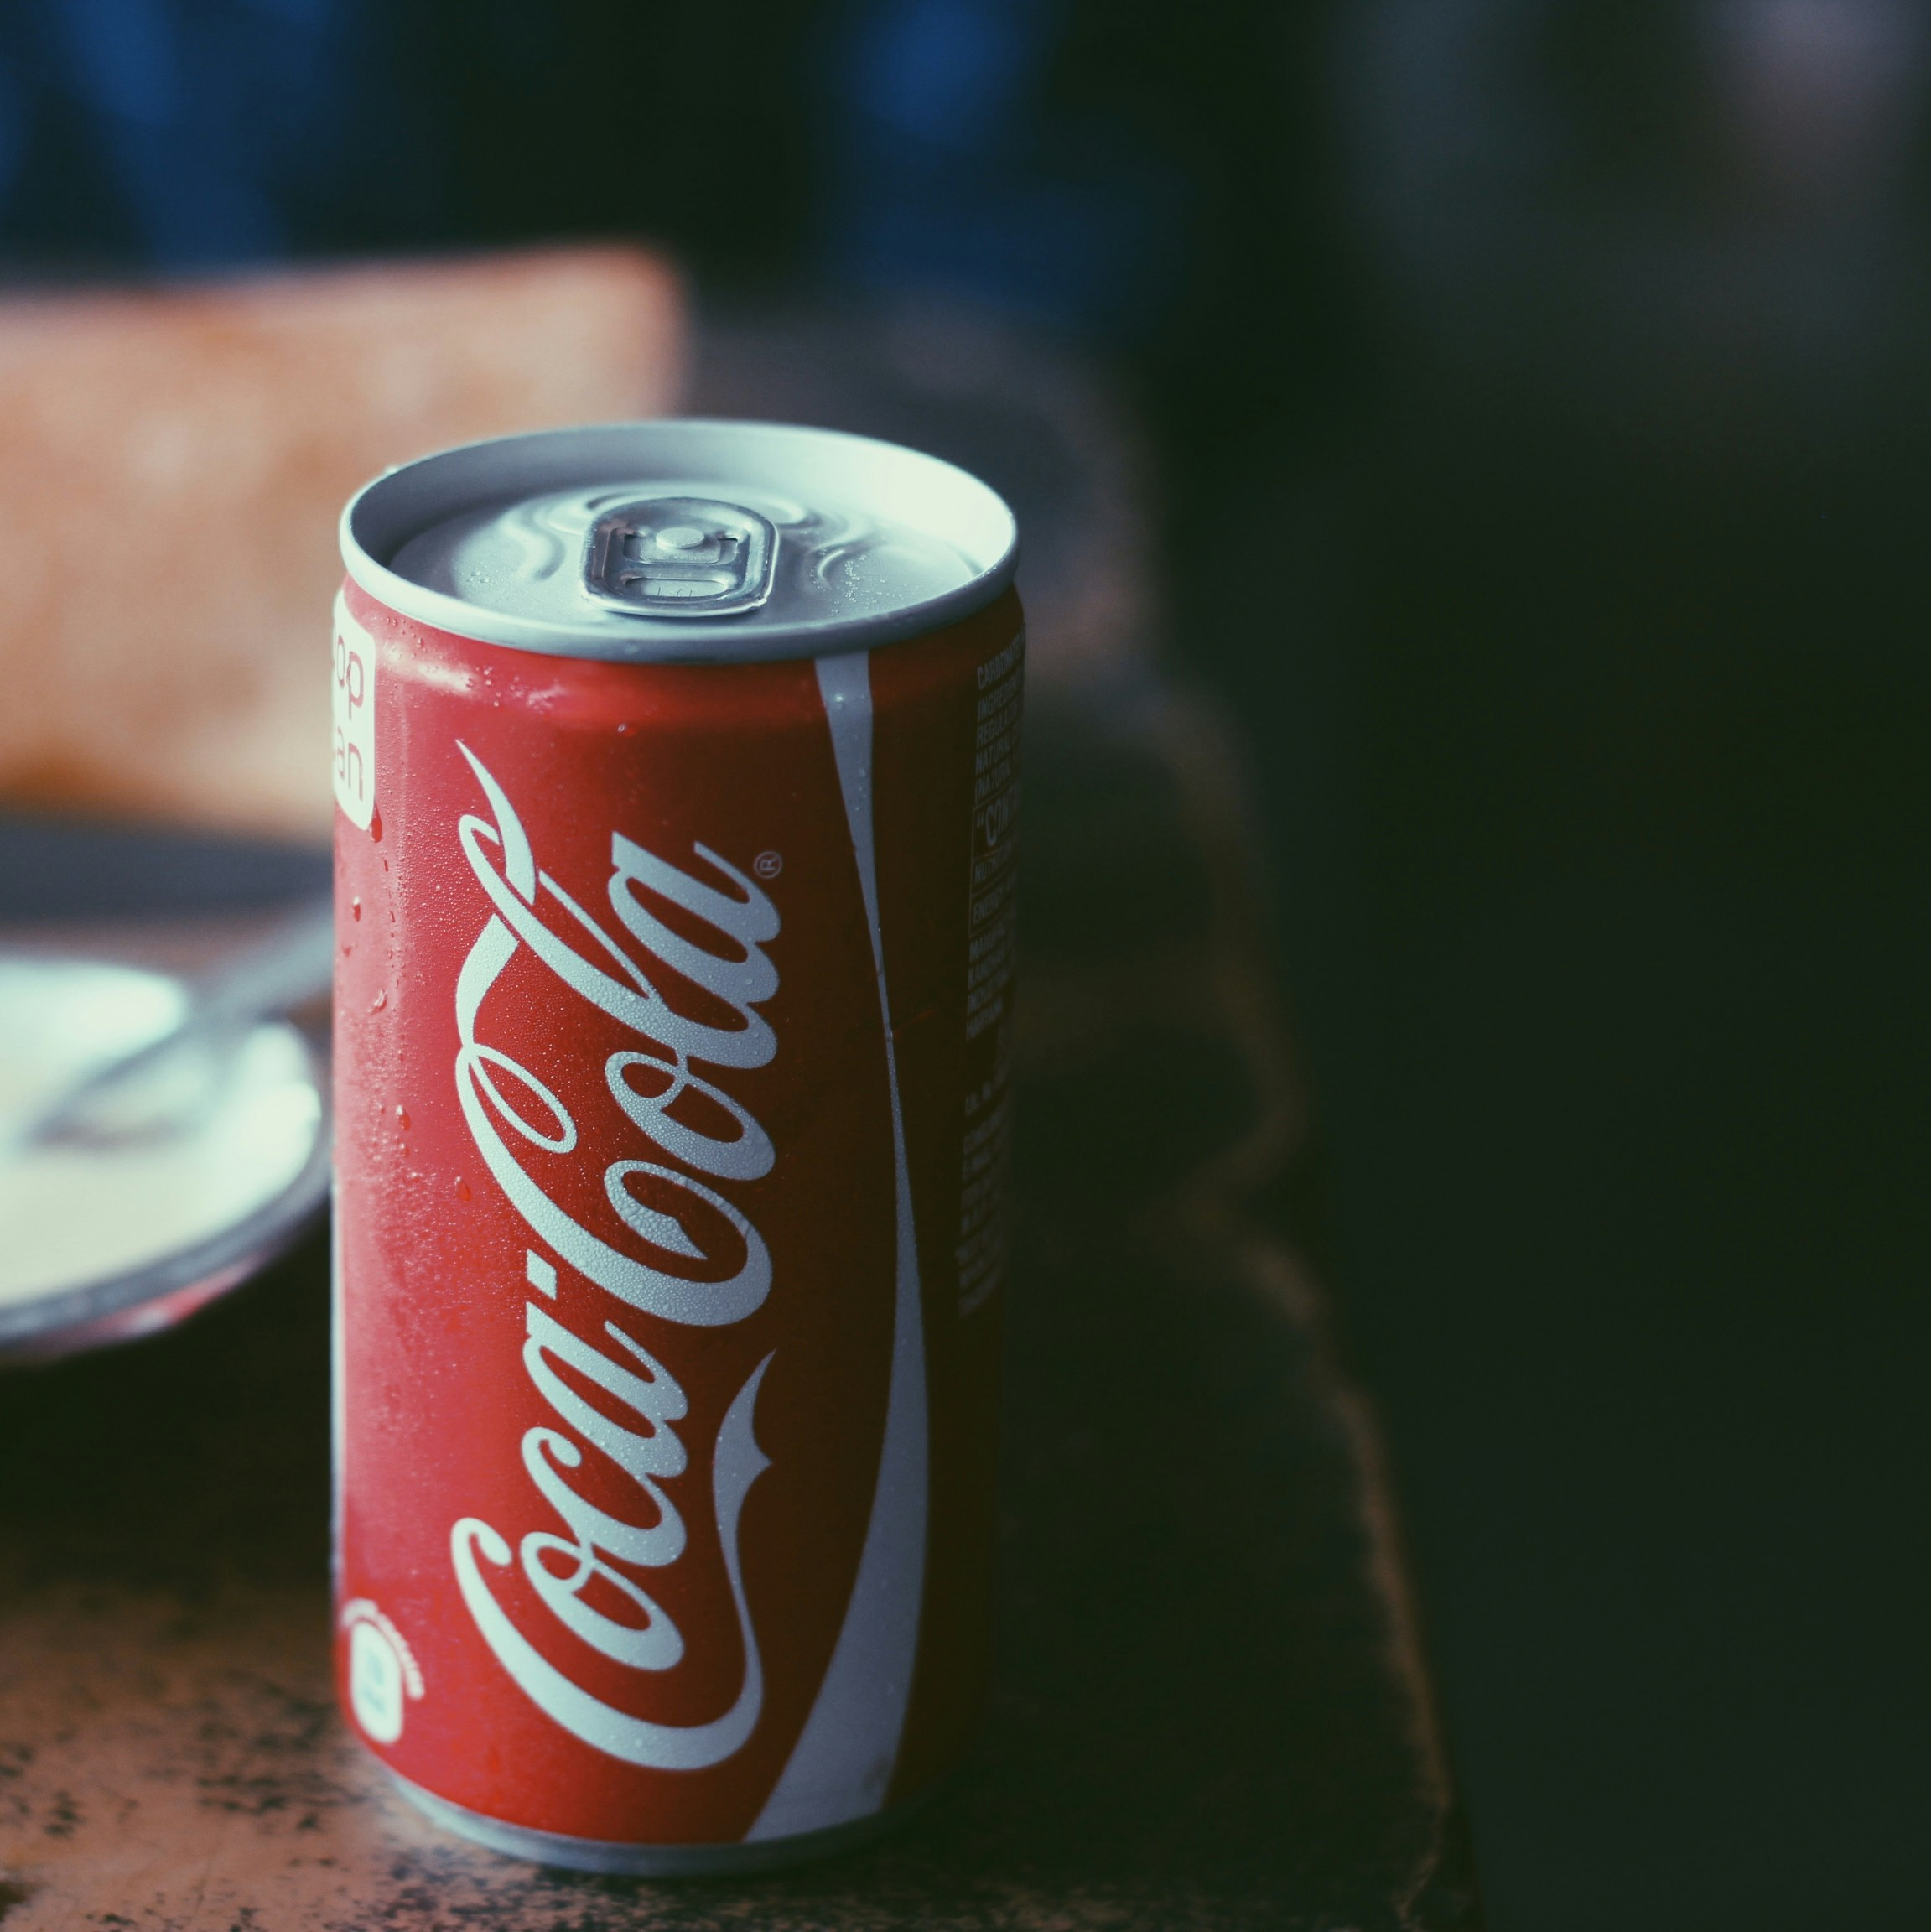
\includegraphics[width = 0.6\textwidth]{Billeder/cola}
	\end{center}
	Vi skal optimere overfladearealet af en cylindrisk dåse. Dåsen skal have et rumfang på 25cm$^2$, og vi
	lader dåsens radius betegnes ved $r$ samt dåsens højde betegnes ved $h$.
\end{opgavetekst}
\begin{delopgave}{}{1}
	Argumentér for, at overfladearealet af dåsen kan beskrives ved 
	\begin{align*}
		O(h,r) = 2 \cdot \pi \cdot r\cdot h + 2 \cdot \pi \cdot r^2
	\end{align*}
	samt at	rumfanget kan beskrives ved 
	\begin{align*}
		R(h,r) =  \pi \cdot r^2 \cdot h
	\end{align*}
\end{delopgave}
\begin{delopgave}{}{2}
	Udnyt at rumfanget af dåsen skal være 250cm$^3$ til at argumentere for, at vi kan skrive overfladearealet 
	som
	\begin{align*}
		O(r) = \frac{500}{r} + 2\cdot \pi \cdot r^2.
	\end{align*}
\end{delopgave}
\begin{delopgave}{}{3}
	Brug differentialregning til at bestemme dimensionerne på dåsen, der giver det mindste overfladeareal. 
\end{delopgave}

\end{document}




